\documentclass[dvipsnames,10pt]{beamer}
\usepackage{ucltemplate}
\usepackage{tikz}
\usetikzlibrary{arrows,shapes, backgrounds, decorations.pathmorphing}
\usepackage{graphicx}
\usepackage{amssymb,amsmath}
\usepackage{listings}
\usepackage{multimedia}
\usepackage{empheq}
\usepackage{makecell}
\usepackage[many]{tcolorbox}
\usepackage[labelformat=empty]{caption,subfig}
%\usepackage[usenames]{color}
%\usetheme{Madrid}
%\mode<presentation>
\setbeamertemplate{navigation symbols}{}
\tikzstyle{na} = [baseline=-.5ex]

\tcbset{highlight math style={enhanced,
  colframe=red!60!black,colback=yellow!50!white,arc=4pt,boxrule=1pt,
  }}

\def\bx{\mathbf{x}}
\def\by{\mathbf{y}}

\renewcommand\theadalign{bc}
\renewcommand\theadfont{\bfseries}
\renewcommand\theadgape{\Gape[4pt]}
\renewcommand\cellgape{\Gape[4pt]}

% From https://tex.stackexchange.com/questions/60216/how-to-create-a-squiggle-arrow-with-some-text-on-it-in-tikz
\newcounter{sarrow}
\newcommand\xrsquigarrow[1]{%
\stepcounter{sarrow}%
\begin{tikzpicture}[decoration=snake]
\node (\thesarrow) {\strut#1};
\draw[->,decorate] (\thesarrow.south west) -- (\thesarrow.south east);
\end{tikzpicture}%
}

\title{Electrostatic simulations with Bempp and Exafmm - A black-box coupling approach}
%\author{\texorpdfstring{Timo Betcke\newline\url{t.betcke@ucl.ac.uk}}{Betcke}}

%\institute[University College London]{Department of Mathematics \\
%  University College London}
\date{}

\begin{document}
\lstset{language=Python}
\tikzstyle{every picture}+=[remember picture]
\begin{frame}
% \vspace*{-0.94cm}
% \hspace*{-1.02cm}
%\noindent\includegraphics[scale=0.4]{1824logo}

% \vspace{-3cm}
\vspace{1cm}

\titlepage
\vspace{-2cm}
\begin{columns}[T]
\begin{column}{.48\textwidth}
\begin{center}
    Timo Betcke \\
    \url{t.betcke@ucl.ac.uk}\\
    University College London
\end{center}
\begin{tcolorbox}
Joint with:\\ Tingyu Wang, Christopher Cooper, and Lorena Barba
\end{tcolorbox}
\end{column}%
\hfill%
\begin{column}{.48\textwidth}
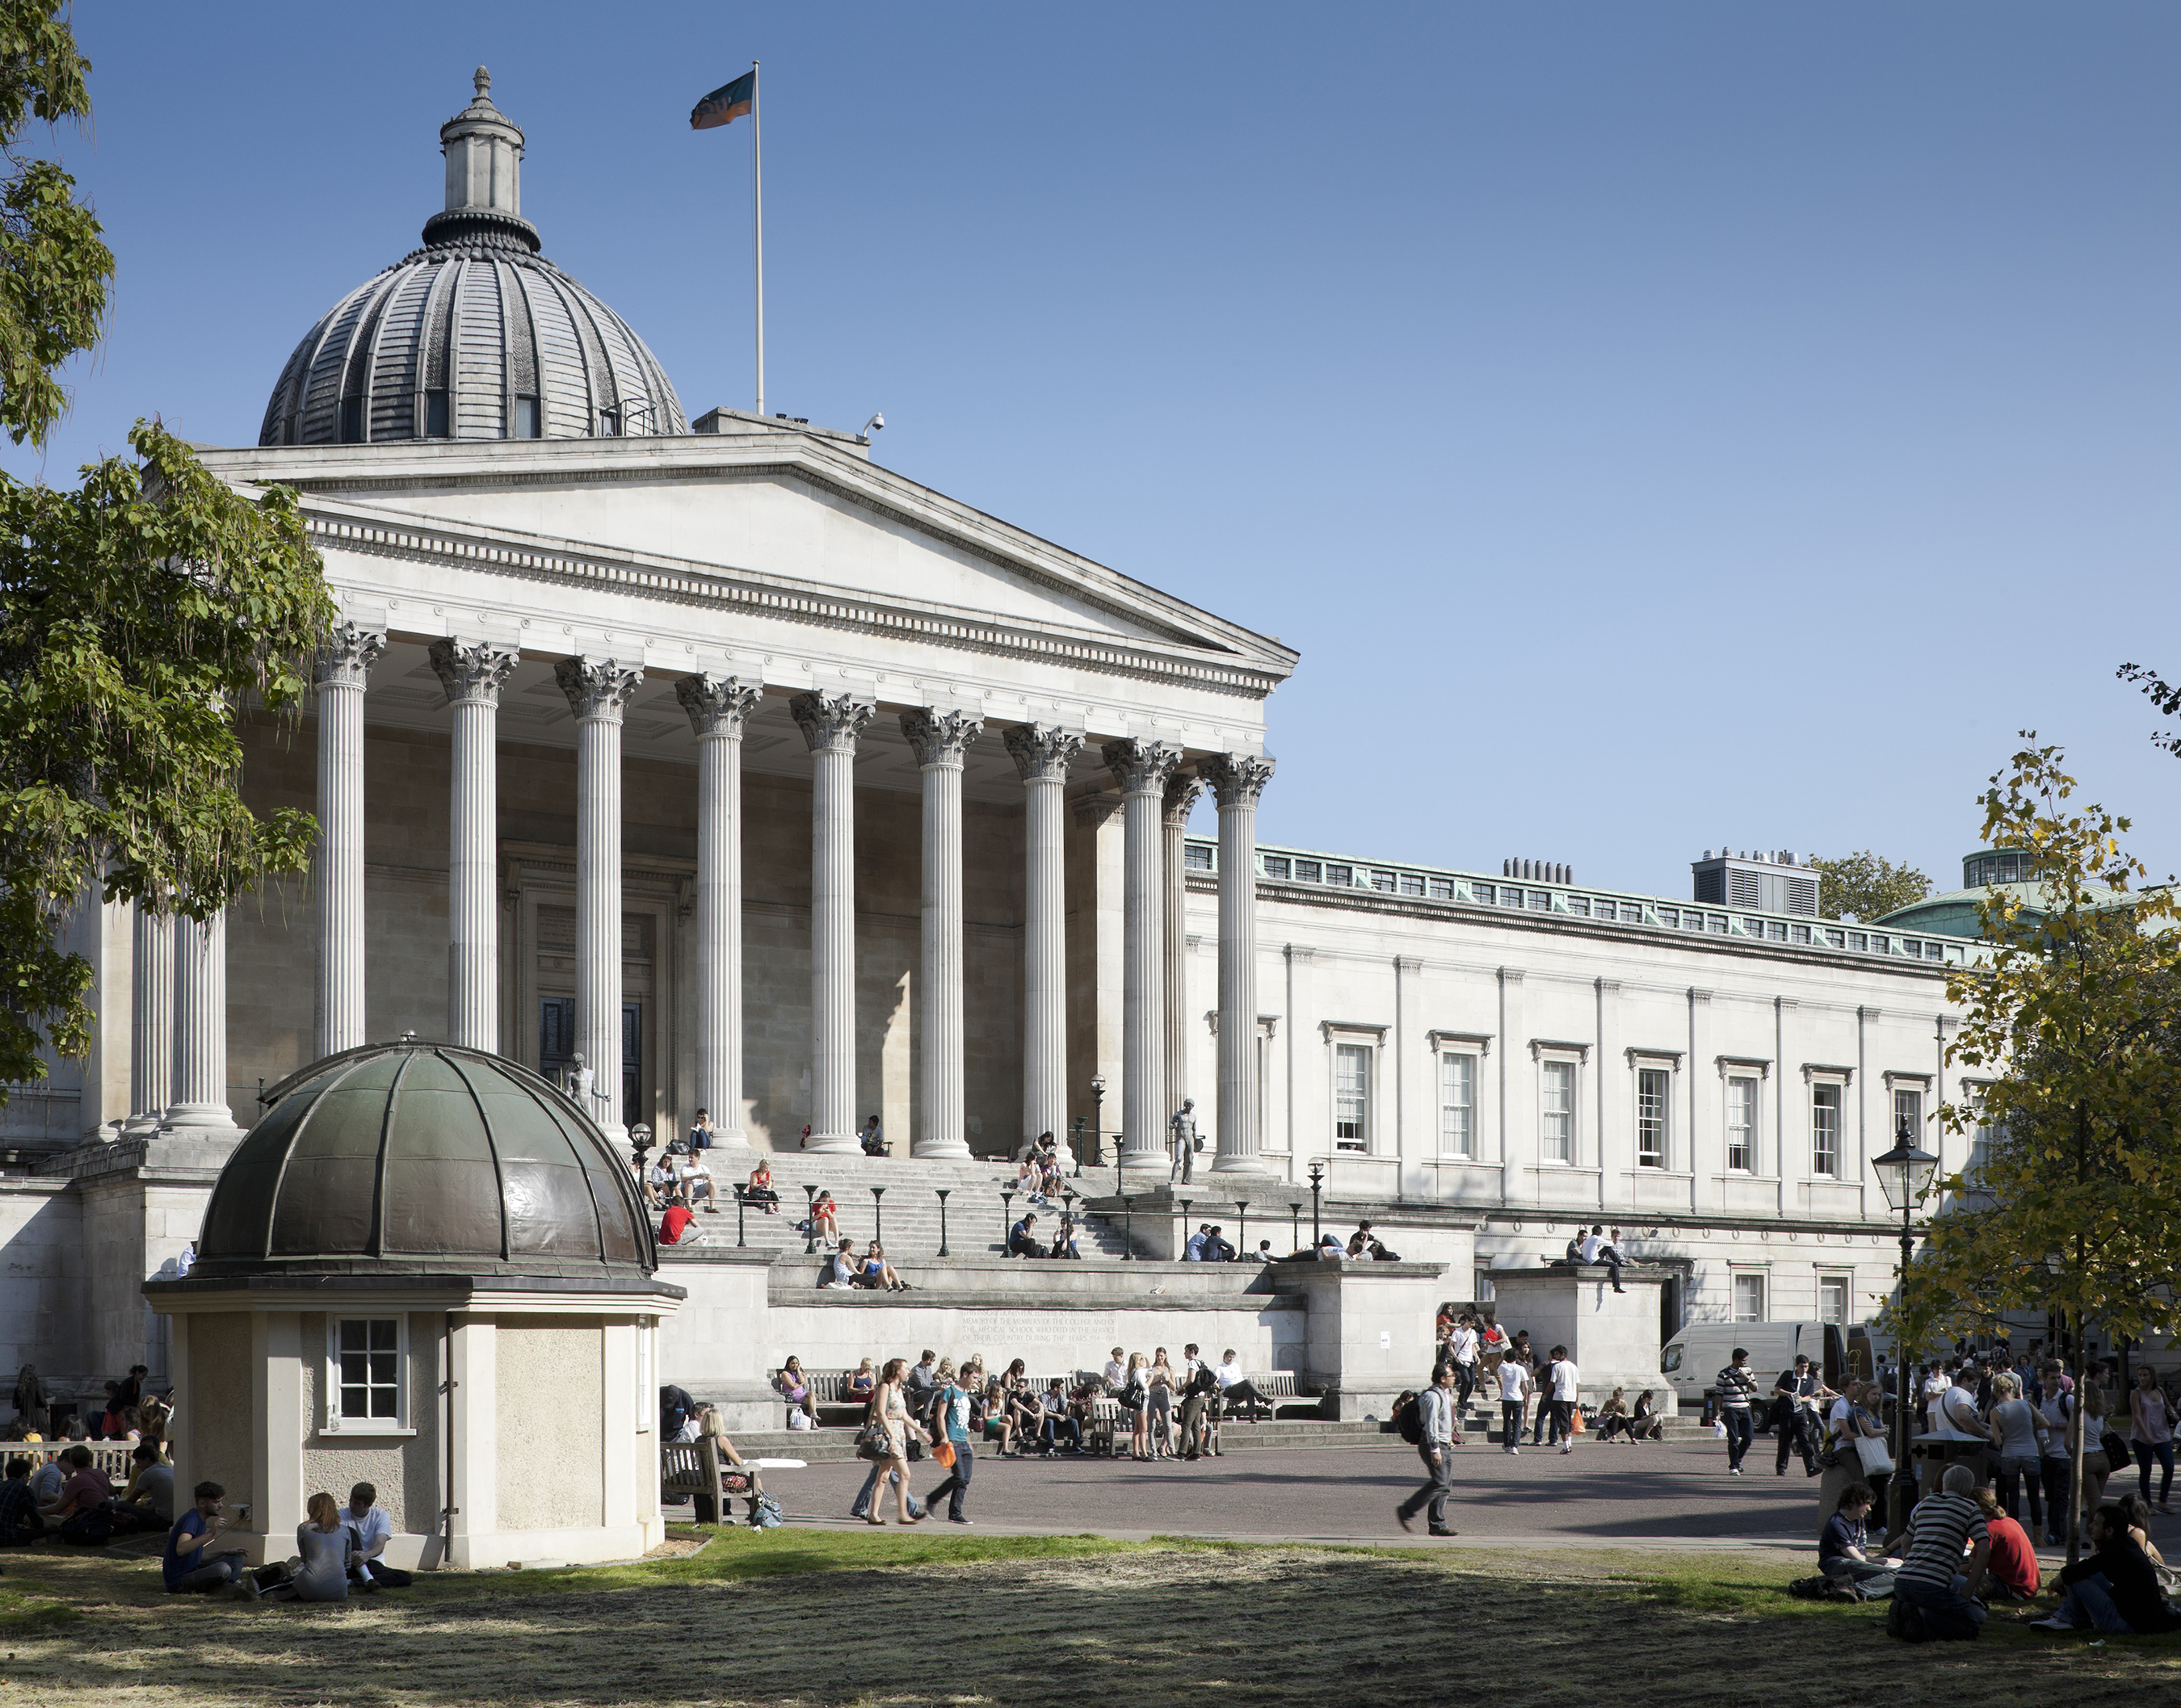
\includegraphics[width=5cm]{../figs/ucl_campus}

\end{column}%
\end{columns}
\textit{Excalibur-SLE: Exascale HPC for System Level Engineering\\
EPSRC Grant: EP/V001531/1}

\end{frame}

\begin{frame}
    \frametitle{Poisson-Boltzmann for virus simulations}

    \vspace{.3cm}

    \begin{minipage}{5cm}
        Solve Poisson-Boltzmann equation
        \begin{align}
            \Delta\phi_1 &= \frac{1}{\epsilon_1}\sum_{k}q_k\delta(\mathbf{r}, \mathbf{r}_k)~\text{in }\Omega_1\nonumber\\
            (\Delta - \kappa^2)\phi_2 &= 0~\text{in }\Omega_2\nonumber
        \end{align}
        Interface conditions on $\Gamma$:
        \begin{align}
            \phi_1 &= \phi_2,\nonumber\\
            \epsilon_1\frac{\partial\phi_1}{\partial\mathbf{n}} &= \epsilon_2\frac{\partial\phi_2}{\partial \mathbf{n}}\nonumber
    \end{align}

    \end{minipage}
    \begin{minipage}{5cm}
        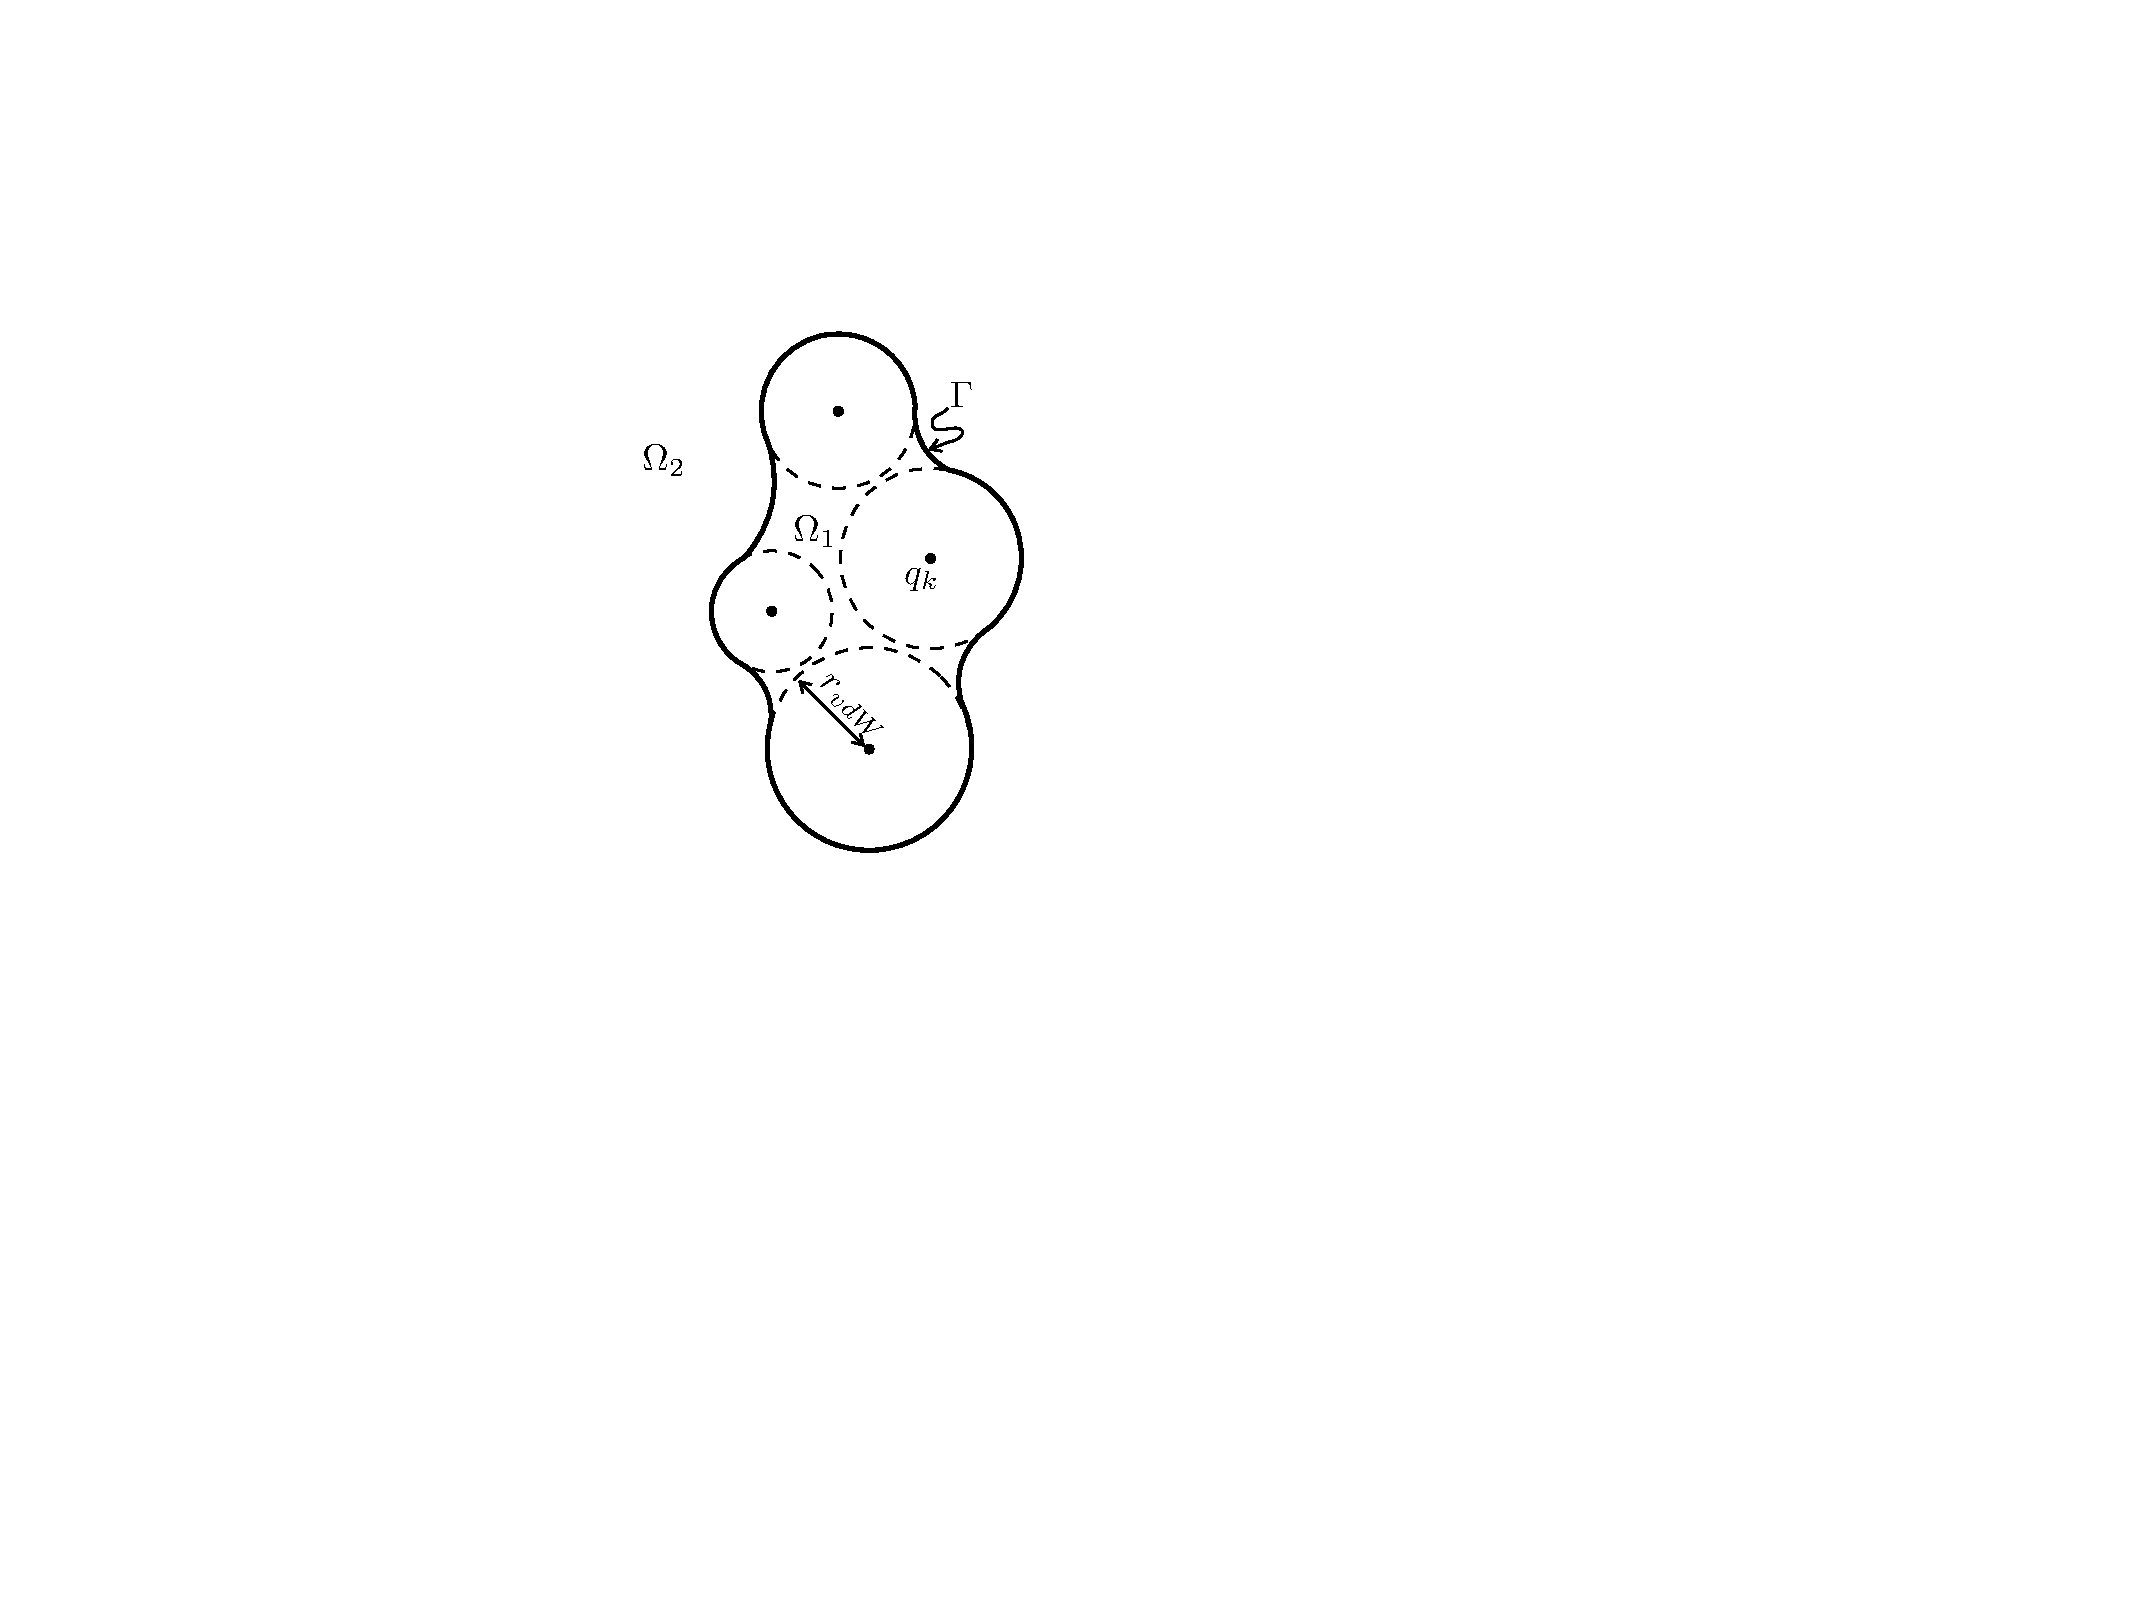
\includegraphics[width=4cm]{../figs/implicit_solvent.pdf}
    \end{minipage}
    Let $\phi_1 = \phi_{reac} + \phi_{coul}$ ($\phi_{coul}$ is potential generated from the point charges only). Then
    want to compute the solvation energy.
    \begin{tcolorbox}
        $$
        \Delta G_{solv}^{polar} = \frac{1}{2}\sum_{k=1}^{N_q}q_k\phi_{reac}(\mathbf{r}_k)
        $$
    \end{tcolorbox}

\end{frame}

\begin{frame}
    \frametitle{Boundary Integral Formulation}

    Exterior field formulation\footnote{Lu et. al., Proc. Natl. Acad. Sci. USA 103 (51) (2006) 19314-19319}
    
\begin{align}
    &\begin{multlined}[t][0.48\textwidth] \frac{\phi_{2,\Gamma}}{2}\left(\frac{\epsilon_1}{\epsilon_2}+1\right) - \left(K_Y^\Gamma - \frac{\epsilon_1}{\epsilon_2}K_L^\Gamma\right)(\phi_{2,\Gamma}) \\
    + \left(V_Y^\Gamma - V_L^\Gamma\right)\left( \frac{\partial}{\partial \mathbf{n}} \phi_{2,\Gamma} \right) = \sum_{k=0}^{N_q}  \frac{q_k}{4\pi\epsilon_2|\mathbf{r}_{\Gamma} - \mathbf{r}_k|}
    \end{multlined} \nonumber \\
    &\begin{multlined}[t][0.48\textwidth] -\frac{\epsilon_1}{\epsilon_2}\left(W_Y^\Gamma - W_L^\Gamma\right)(\phi_{2,\Gamma}) +  \frac{1}{2}\frac{\phi_{2,\Gamma}}{\partial\mathbf{n}}\left(1+\frac{\epsilon_1}{\epsilon_2}\right) \\
    + \left(\frac{\epsilon_1}{\epsilon_2}K_Y^{\prime\Gamma} - K_L^{\prime\Gamma}\right)\left( \frac{\partial}{\partial \mathbf{n}} \phi_{2,\Gamma} \right) = \sum_{k=0}^{N_q}  \frac{\partial}{\partial\mathbf{n}_\mathbf{r}}\left(\frac{q_k}{4\pi\epsilon_2|\mathbf{r}_{\Gamma} - \mathbf{r}_k|}\right)\nonumber
    \end{multlined}
\end{align}

Also possible to derive interior field formulation (due to Juffur) or simple 
direct coupling from first line of Calder\`{o}n projector. 
Exterior formulation most favourable in terms of conditioning.

\end{frame}

\begin{frame}
    \frametitle{Zika virus}
    \begin{minipage}{6cm}
        \begin{itemize}
            \item Around 1.6m atoms
            \item Generated mesh has around 10m surface elements
        \end{itemize}
    \end{minipage}
    \begin{minipage}{4cm}
        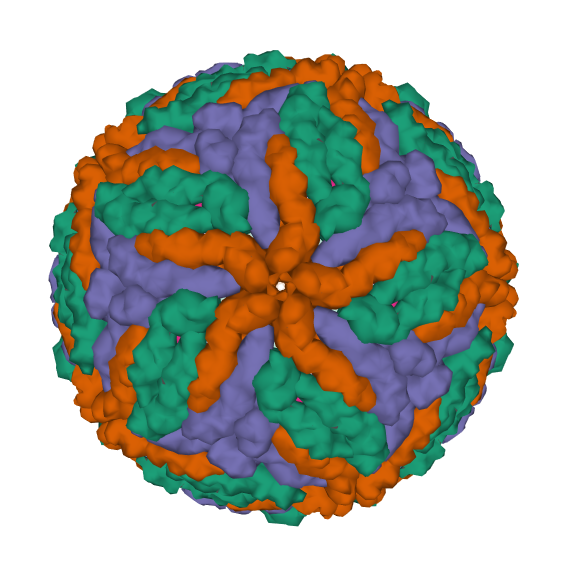
\includegraphics[width=4cm]{../figs/6CO8_assembly.png}
    \end{minipage}

\begin{tcolorbox}
    Use Galerkin BEM code Bempp-cl accelerated with fast particle interactions through Exafmm
\end{tcolorbox}

Outline of rest of talk:
\begin{itemize}
    \item A short introduction to Bempp-cl and Exafmm
    \item Black-box coupling strategies for Galerkin BEM
    \item Practical issues and ongoing work
\end{itemize}

\end{frame}

\begin{frame}
    \frametitle{Bempp-cl}
    \begin{itemize}
        \item Successor of the Bempp boundary element library.
        \item Fully developed using Python with fast OpenCL kernels for computational routines.
        \item Galerkin discretisation of operators for Laplace, Helmholtz, and Maxwell problems.
        \item Compute kernels can be run on CPU or offloaded to GPU.
        \item Core routines optimised for fast dense assembly of opertors.
        \item Library provides coupling interfaces to Exafmm, can be easily adapted to other
            fast particle summation libraries.
    \end{itemize}
\end{frame}

\begin{frame}
    \frametitle{Characteristics of Bempp-cl}
    \vspace{-.1cm}
    \begin{center}
        \begin{tabular}{cc}
            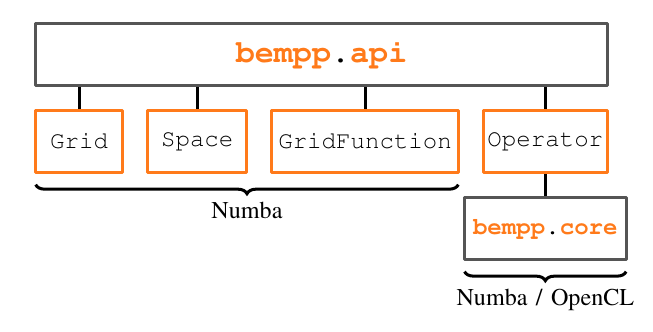
\includegraphics[width=5cm]{../figs/bempp_cl_overview.png} & 
            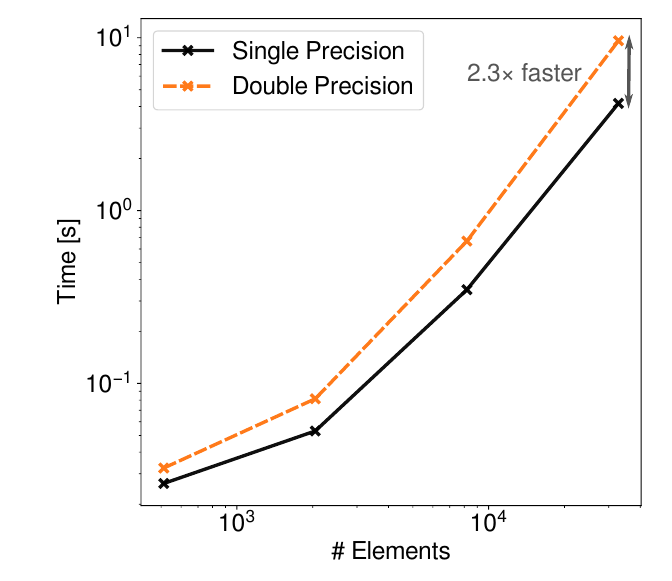
\includegraphics[width=5cm]{../figs/bempp_single_vs_double.png} \\
            \begin{minipage}{5cm}
                \vspace{-4cm}
                \begin{itemize}
                    \item Top: Structure of Bempp-cl
                    \item Top-Right: AVX acceleration in Bempp-cl
                    \item Bottom-Right: Offloading of a domain potential operator
                \end{itemize}
            \end{minipage}&
            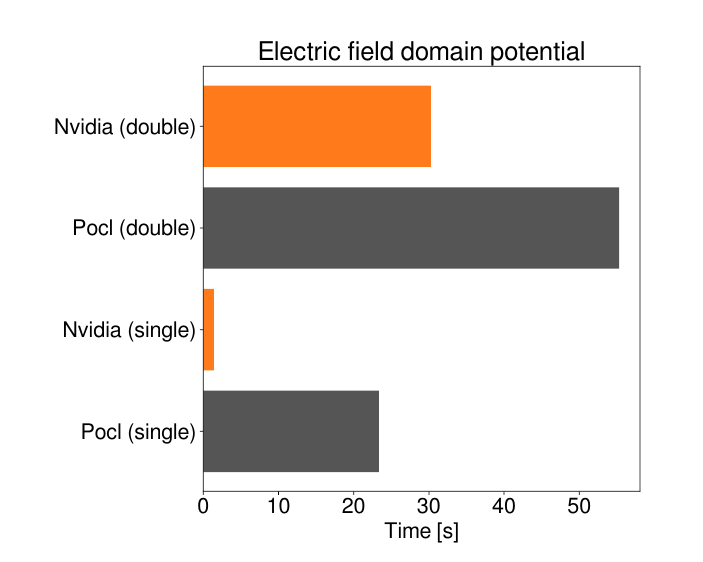
\includegraphics[width=5cm]{../figs/gpu_offloading.png} 
        \end{tabular}
    \end{center}
\end{frame}

\begin{frame}
    \frametitle{Exafmm-t: High-Performance KIFMM}
    \vspace{-.1cm}
    \begin{center}
        \begin{tabular}{cc}
            \begin{minipage}{5cm}
                \begin{itemize}
                    \item Kernel-Independent FMM library.
                    \item Written in C++, Provides Python Interface.
                    \item Highly efficient at higher accuracies.
                \end{itemize}
            \end{minipage} &
            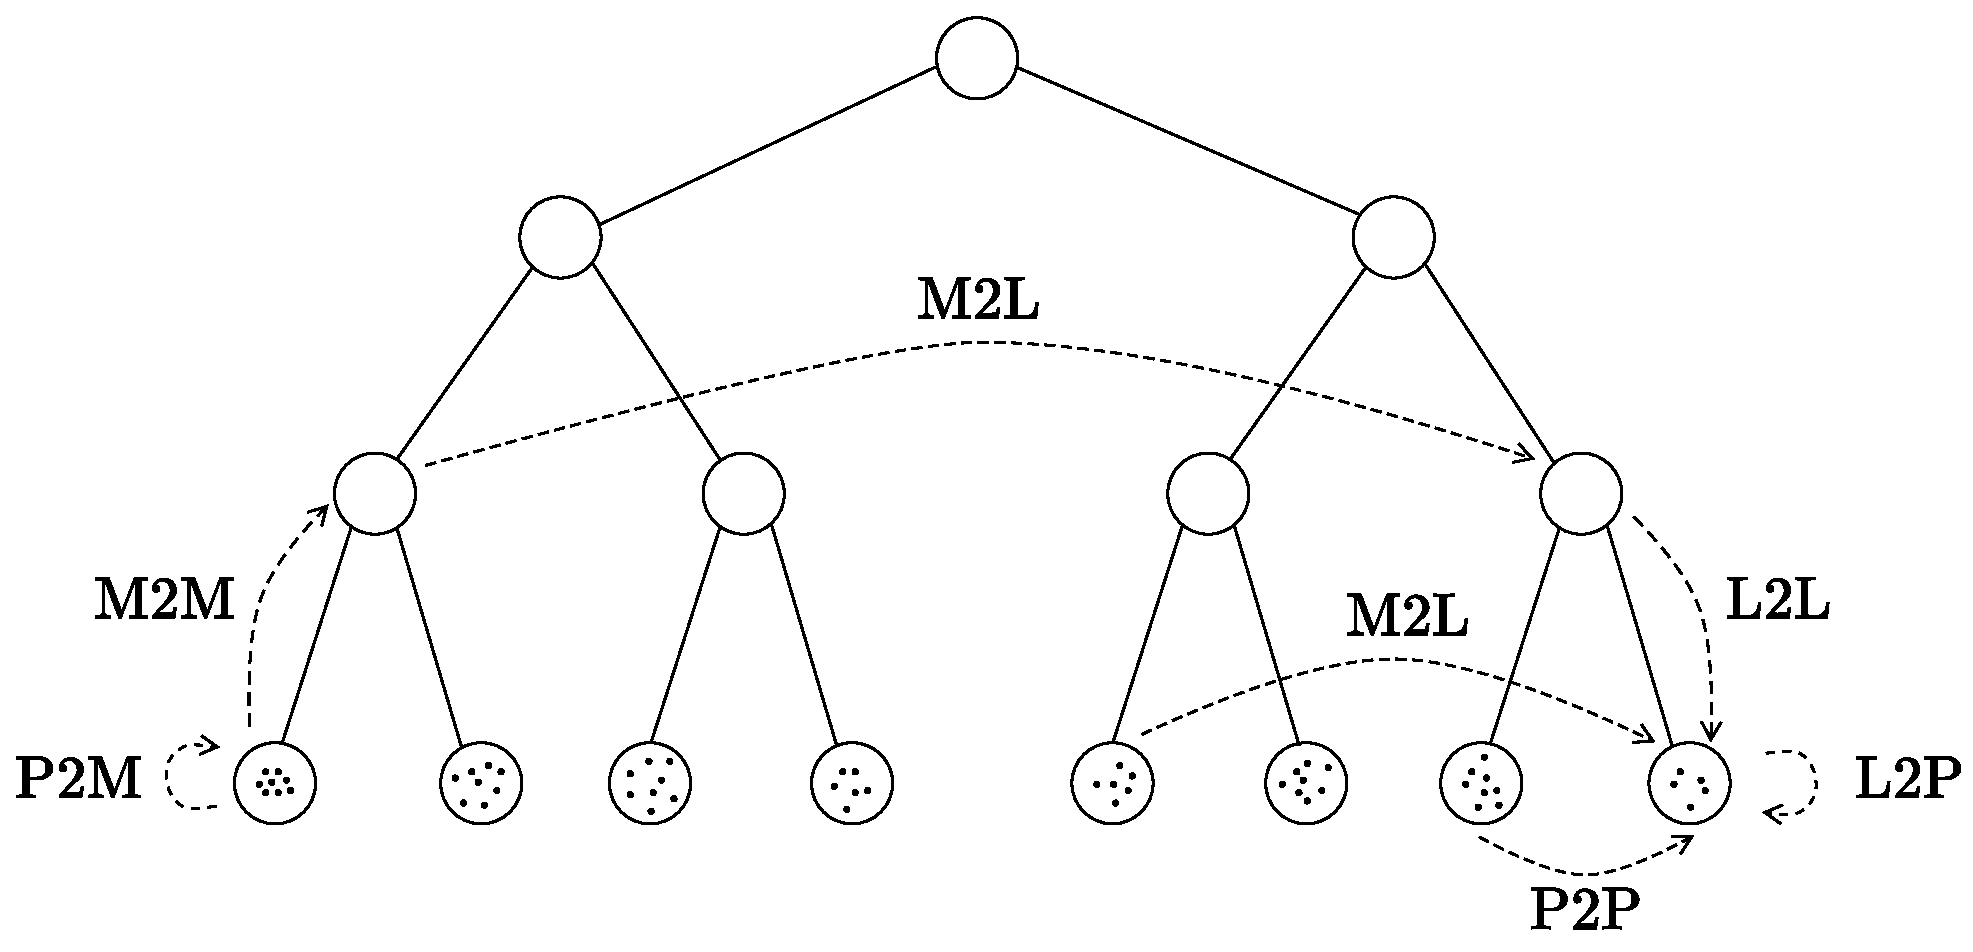
\includegraphics[width=5cm]{../figs/fmm_sketch.pdf} \\
            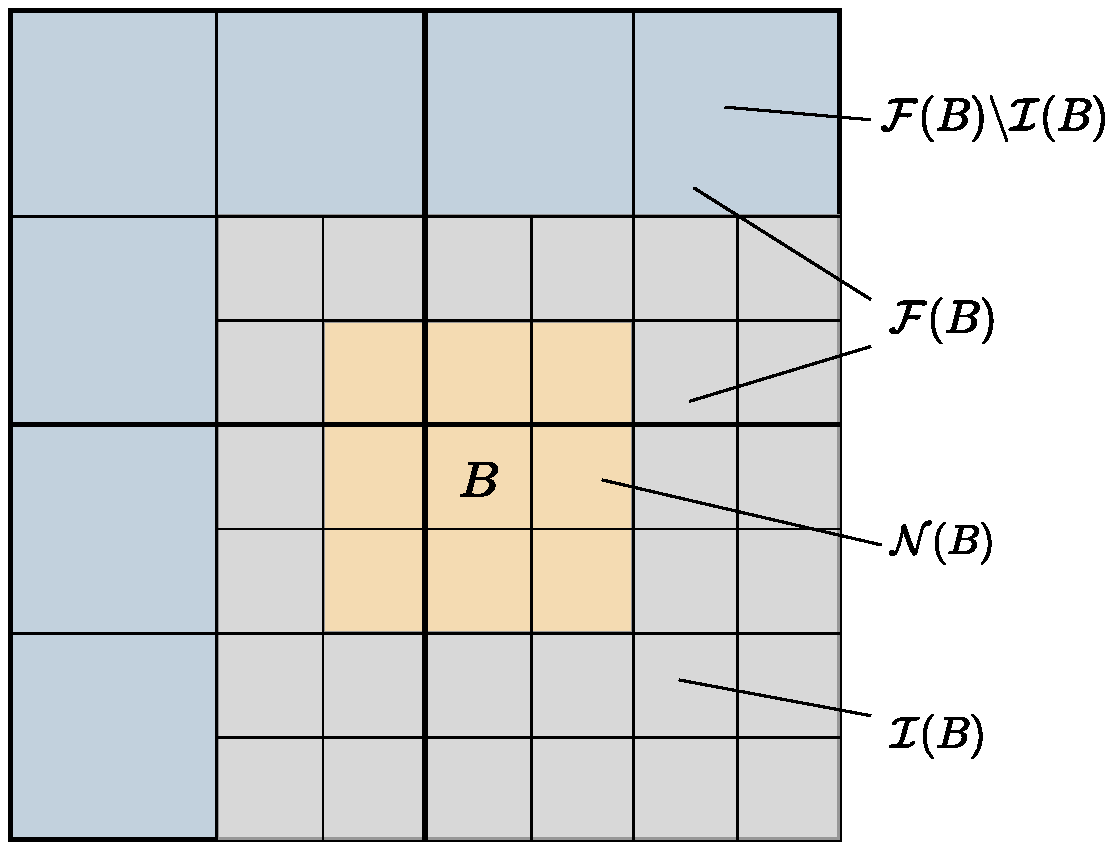
\includegraphics[width=4cm]{../figs/near_far_decomposition.pdf} &
            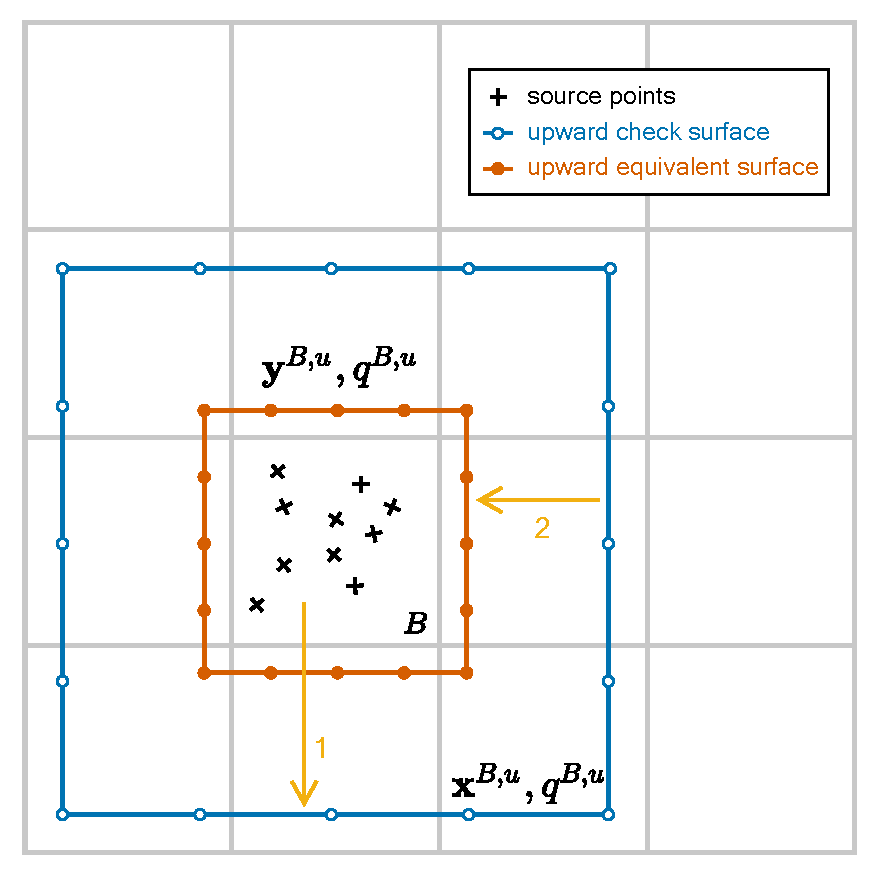
\includegraphics[width=4cm]{../figs/multipole_expansion.pdf}
        \end{tabular}
    \end{center}

\end{frame}
    
\begin{frame}
    \frametitle{Coupling Bempp-cl and Exafmm-t}

Let $A$ be the matrix representation of a Galerkin discretised boundary integral operator.
Let $x$ be any vector. Reformulate $Ax$ as

$$
Ax = P_{test}^T(G - C)P_{dom}x + Sx
$$

\begin{itemize}
    \item $P_{test}$ and $P_{dom}$ highly sparse matrices that map function space coefficients to particle weights at quadrature points.    \item $G$ is black-box operator evaluating particle sums over weights across all quadrature points across all elements.
    \item $C$ is sparse matrix that contains the particle interactions between neighboring triangles.
    \item $S$ is sparse matrix containing all singular Galerkin integrals in adjacent elements.
\end{itemize}

\end{frame}

\begin{frame}
    \frametitle{The correction matrix}

    \begin{center}
        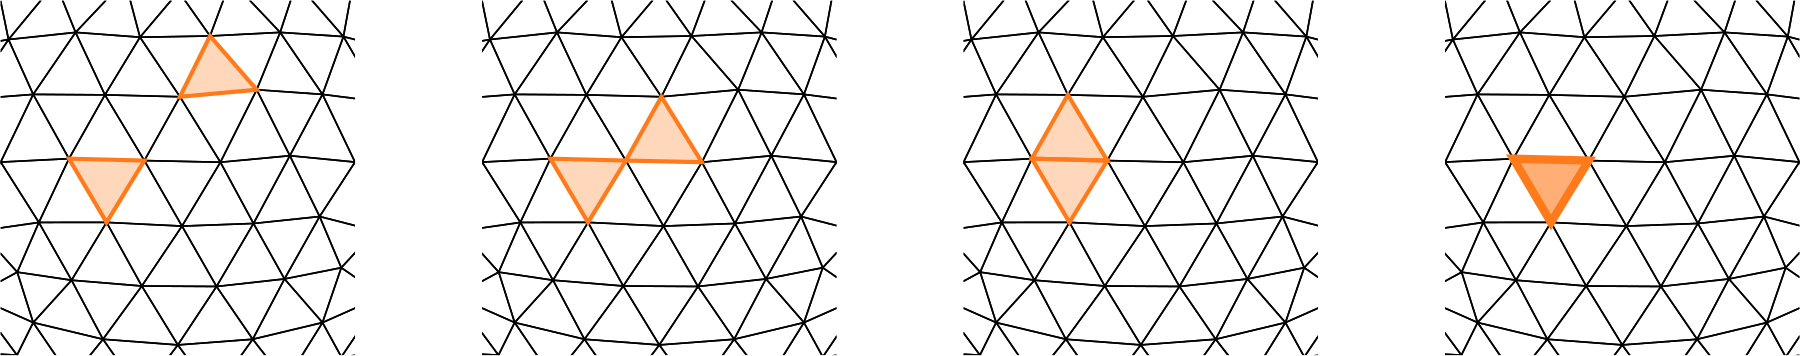
\includegraphics[width=10cm]{../figs/triangles.png}
    \end{center}

    Problem: Any FMM code also evaluates the near-field.
    Near-field can contain adjacent triangles (singular quadrature rules), and
    non-adjacent triangles (standard triangle Gauss rule).

    \vspace{.5cm}

    The sources and target points in the FMM are arising from the
    non-singular quadrature rule.

    \vspace{.5cm}

    Solution: After FMM evaluation subtract out the regular quadrature rule
    contribution from adjacent triangles and add in the correct singular quadrature
    rule contribution.

\end{frame}

\begin{frame}
    \frametitle{Number of FMM passes per Operator}

    \begin{tabular}{c|c|c|c|c}
        Operator & $V$ & $K$ & $K'$ & $W_Y$, $W_L$ \\
        \hline
        FMM Passes & 1 & 3 & 1 & 6, 3 
    \end{tabular}

    \vspace{.5cm}

    Example: Double-Layer Potential Operator

    \begin{align}
        [K\phi](\mathbf{x}) &= \int_{\Gamma}
        \partial_{\mathbf{n(\mathbf{y})}}g(\mathbf{x}, 
        \mathbf{y})\phi(\mathbf{y})ds(\mathbf{y})\nonumber \\
        &= -\sum_{j=1}^3\left[\nabla_{\mathbf{x}} 
        g(\mathbf{x}, \mathbf{y})\right]_j\mathbf{n}_j(\mathbf{y})
        \phi(\mathbf{y})ds(\mathbf{y})\nonumber
\end{align}

Require three FMM passes for the three different densities $\tilde{\phi}_j(\mathbf{y}):=\mathbf{n}_j(\mathbf{y})\phi(\mathbf{y})$, $j=1,\dots, 3$.

\vspace{.5cm}

The transmission operator for the exterior Poisson-Boltzmann formulation requires {\color{red} 19 FMM passes}.

\end{frame}

\begin{frame}
    \frametitle{Poisson-Boltzmann for a sphere}

    \begin{center}
        \begin{tabular}{cc}
            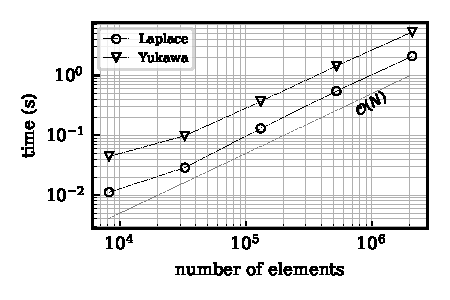
\includegraphics[width=5cm]{../figs/sphere_fmm.pdf} &
            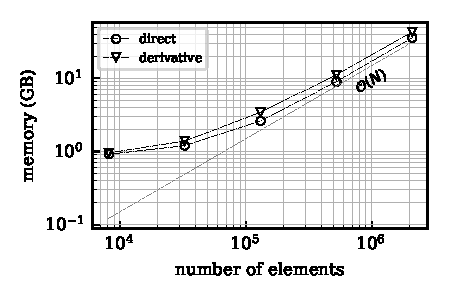
\includegraphics[width=5cm]{../figs/sphere_memory.pdf} \\
            \begin{minipage}{5cm}
                \vspace{-3.5cm}
                \begin{itemize}
                    \item FMM Expansion Order 5
                    \item 6 regular quadrature points per element
                    \item \textbf{Right} Blue: Laplace, 
                        Yellow: Yukawa, Green: Singular Correction, Red: Other
                \end{itemize} 
            \end{minipage} &
            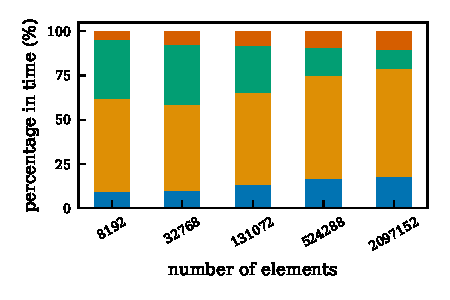
\includegraphics[width=5cm]{../figs/sphere_gmres_derivative.pdf}
        \end{tabular}
    \end{center}
\end{frame}

\begin{frame}
    \frametitle{Results for Zika Virus}

    \begin{center}
        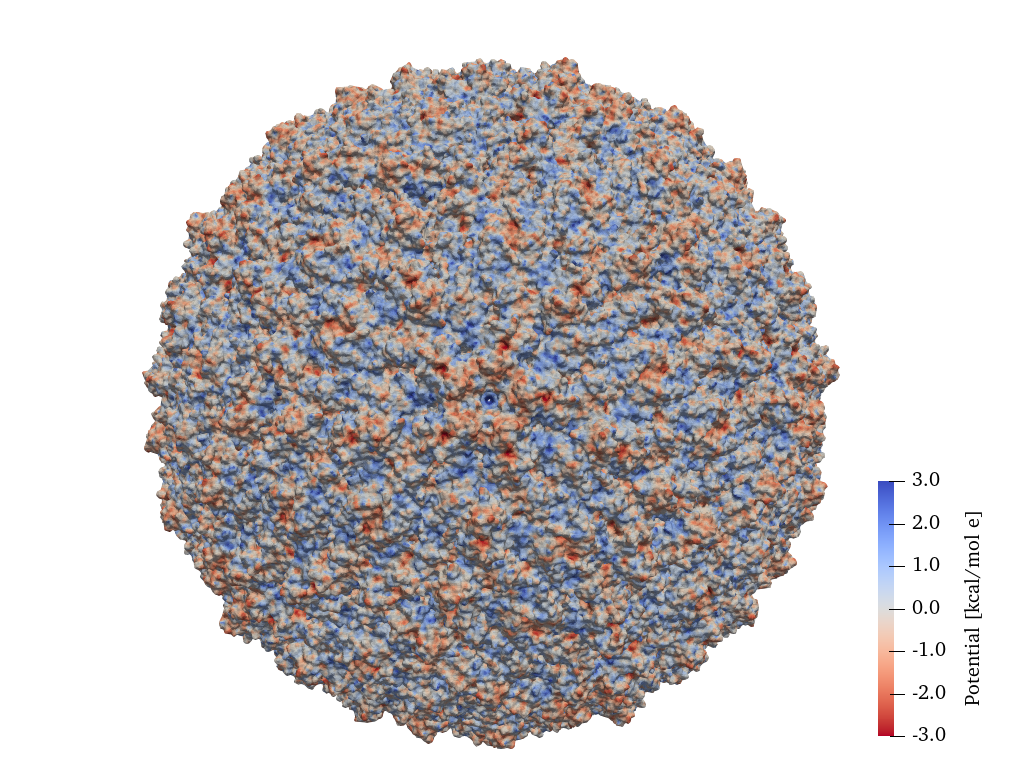
\includegraphics[width=8cm]{../figs/6CO8_potential.png}
    \end{center}

    40 Core Compute node. Total time: 139.5 minutes, GMRES time: 80 minutes, 18 GMRES iterations, Max RAM use: 43GB, $\Delta G_{solv} = -116254.9 kcal/mol$. Diagonal preconditioner through inverse of mass matrix with mass lumping.

\end{frame}

\begin{frame}
    \frametitle{FMM - The next steps}

    {\color{blue} PyExafmm - KIFMM in Python}

    \vspace{\baselineskip}

    \begin{itemize}
        \item Provide a hackable and performant Adaptive FMM in Python.
        \item Test bed for further developments.
        \item Far-field computation accelerated through Numba.
        \item Randomized compression of M2L operators.
    \end{itemize}

    \vspace{\baselineskip}

    {\color{blue}\url{https://github.com/exafmm/pyexafmm}}

\end{frame}

\begin{frame}
    \frametitle{A Rust based scalable fast solver framework}

    \vspace{.2cm}
    Goal: Create a fast solver framework for fast parallel forward evaluation and
    approximate inversion of integral operators (\url{https://github.com/rusty-fast-solvers/roadmap})

    \vspace{\baselineskip} 

    {\color{blue} All component libraries developed in Rust with Rayon (multithreading)
    and MPI (across nodes) for parallelization.}
    \vspace{\baselineskip}

    Development Status:
    \begin{itemize}
    \item {\color{blue} rusty-green-kernel} AVX accelerated direct evaluation
        of Laplace, Helmholtz Green's functions. {\color{green} Usuable}.
    \item {\color{blue} rusty-tree} Serial and parallel Octree implementations.
        Serial tree implemented. 
        Parallel tree early stages. {\color{yellow} Partially implemented}.
    \item {\color{blue} rusty-compression} Fast randomized compression routines
        for approximate low-rank matrices. {\color{yellow} Mostly finished.}
    \item {\color{blue} rusty-translation} Implementation of M2M, 
        M2L, L2L, P2M, L2P operators
        based on numerical field compressions (KIFMM, etc.)
        {\color{red} In planning}
    \item {\color{blue} rusty-fmm} Serial and parallel FMM loops 
        {\color{red} In planning}
    \item {\color{blue} rusty-inverse} Evaluation of approximate inverses 
        {\color{red} Not yet started}
    \end{itemize}

\end{frame}

\begin{frame}
    \frametitle{Summary}

    \begin{itemize}
        \item Generic, practically usuable and efficient black-box coupling of Galerkin
            BEM and Exafmm.
        \item All computational results shown today steered through interactive Jupyter
            notebooks.
        \item Python glue language between the codes. High productivity through Jupyter
            interface.
        \item For links to paper, reproducible data and codes see\\
            \url{https://github.com/barbagroup/bempp_exafmm_paper}
    \end{itemize}

    \begin{tcolorbox}
        Work supported through Exalibur-SLE: Exascale HPC for System Level Engineering 
    \url{https://excalibur-sle.github.io/}
    \end{tcolorbox}

\end{frame}

\begin{frame}
    \frametitle{Papers}

{
    \small

\begin{itemize}
    \item T. Wang, C. Cooper, T. Betcke, L. Barba, \textit{High-productivity, 
        high-performance workflow for virus-scale electrostatic simulations with 
    Bempp-Exafmm}, arXiv preprint arXiv:2103.01048 (2021), 
    \url{https://github.com/barbagroup/bempp_exafmm_paper}
    \item T. Betcke, M. W. Scroggs, \textit{Bempp-cl: A fast Python based 
        just-in-time compiling boundary element library}, 
        Journal of Open Source Software, 6(59), 2879 (2021), 
            \url{https://doi.org/10.21105/joss.02879}
    \item T. Betcke, M. W. Scroggs, \textit{Designing a high-performance boundary 
        element library with OpenCL and Numba}, 
        Computing in Science \& Engineering, to appear (2021) 
        \url{https://doi.org/10.1109/MCSE.2021.3085420} 
    \item T. Wang, R. Yokota, L. Barba, \textit{ExaFMM: a high-performance 
            fast multipole method library with C++ and Python interfaces.}
        Journal of Open Source Software, 6(61), 3145 (2021),
        \url{https://doi.org/10.21105/joss.03145}
    \end{itemize}

}


    \vspace{1cm}


\end{frame}

\end{document}

